\chapter{Analysis and Design}
\label{chap:analysis-design}

Leveraging the notions coming from \Cref{chap:background}, this chapter inspects the current state of aggregate computing, identifying some of the missing features of the current model as proposed by field calculus (\Cref{sec:current-state}).
%
Subsequently, \Cref{sec:proposed-model} describes a prototype of a \textit{reactive model} for aggregate computing, introducing the objectives and giving a preliminary analysis of how the proposed model is expected to fulfill them.
%
Finally, \Cref{sec:design} presents the major design choices that were taken prior to implementation.

\section{Analysis of the current state}
\label{sec:current-state}

In order to have a comprehensive view on the subject, this section provides a brief analysis of the current state of aggregate computing, first by describing the \textit{proactive model} and identifying its limitations, then by introducing \textit{ScaFi}

\subsection{Proactive model}

At the current stage, field calculus and aggregate computing are based on a model where each device of the network \textit{repeatedly} executes its computation in rounds of \textit{sense-eval-broadcast}.
%
In particular, referring to the model discussed in \cite{10.1145/3177774}, each sense-eval-broadcast round of a device is alternated with some \textit{sleeping time} during which it collects information from neighboring devices.
%
This way of managing computation can be thought of as a \textit{proactive model}, since its the device that decides when computation should occur based on its internal scheduler.

The proactive model has some shortcomings.
%
On the one hand, there is no way to granularly control the \textit{timing} and the \textit{dynamics} of computation rounds using the main operators of field calculus alone.
%
In fact, there is often the need to perform computation upon the occurrence of particular events, for example when a sensor changes its value, or when a message is received from a neighbor.

On the other hand, since computations are carried out regardless of the existence of significant changes in the environment or in the knowledge of the neighborhood.
%
In turn, this implies that the \textit{broadcast} step is also carried out even if there is no change in the generated export, resulting in \textit{wasteful message exchange}.

The shortcomings of the proactive model call for a more \textit{reactive approach}, where taking actions only upon significant changes is a pivotal concern and should be taken into account as first class in the supporting model.
%
A prototype for this is presented in \Cref{sec:proposed-model}.

\subsection{ScaFi}

This section presents a brief introduction to \textbf{ScaFi}, a Scala-based library and framework for aggregate programming \cite{scafi-docs}.
%
In particular, the \textit{API} and the \textit{core} of ScaFi will be analyzed in order to facilitate both the design and implementation stages, since they can be used as references to guide the whole process.

ScaFi's API is heavily inspired by the field calculus' language and consists of a trait defining the main constructs that can be used to describe aggregate computations:
%
\begin{lstlisting}[frame=single, language=scala]
trait Constructs {
  def nbr[A](expr: => A): A
  def rep[A](init: =>A)(fun: (A) => A): A
  def foldhood[A](init: => A)(aggr: (A, A) => A)(expr: => A): A
  def aggregate[A](f: => A): A
  def align[K,V](key: K)(comp: K => V): V

  def mid(): ID
  def sense[A](name: CNAME): A
  def nbrvar[A](name: CNAME): A
}
\end{lstlisting}
%
Some notes to keep in mind about ScaFi's API are:
%
\begin{itemize}
    \item an expression written using the API is evaluated by each device once per computation round;
    \item fields are represented as \textit{atomic values} (i.e. they have no particular wrapper around them) and they indicate the value of the field at the device performing that computation;
    \item \texttt{sense} evaluates the sensor with the given \texttt{name}, effectively producing a field of the requested sensor value;
    \item \texttt{nbrvar} is a mechanism to perform a query against a neighboring sensor with a given \texttt{name};
    \item the concept of neighboring field from field calculus is not \quotes{reified}, meaning that there is no actual data structure representing it; spatial computation (i.e. the \texttt{nbr} and \texttt{nbrvar} constructs) is only available inside a special scope, given by the \texttt{foldhood} construct;
    \item \texttt{foldhood} acts in such a way that the \texttt{expr} parameter is evaluated for each aligned neighbor (internally constructing the neighboring field) and the final output is obtained by \textit{folding} all neighboring values using \texttt{init} and \texttt{aggr};
    \item the export for each iteration is constructed by the \textit{engine} of ScaFi, by applying side-effects to an internal data structure as these constructs get invoked, therefore constructing the evaluation tree.
\end{itemize}

This API can be used to implement an idiomatic building block of aggregate computing, which is known as \textit{gradient}.
%
A gradient is a numerical field that expresses the minimum distance from any device to source devices (\Cref{fig:gradient}).
%
\begin{figure}
    \centering
    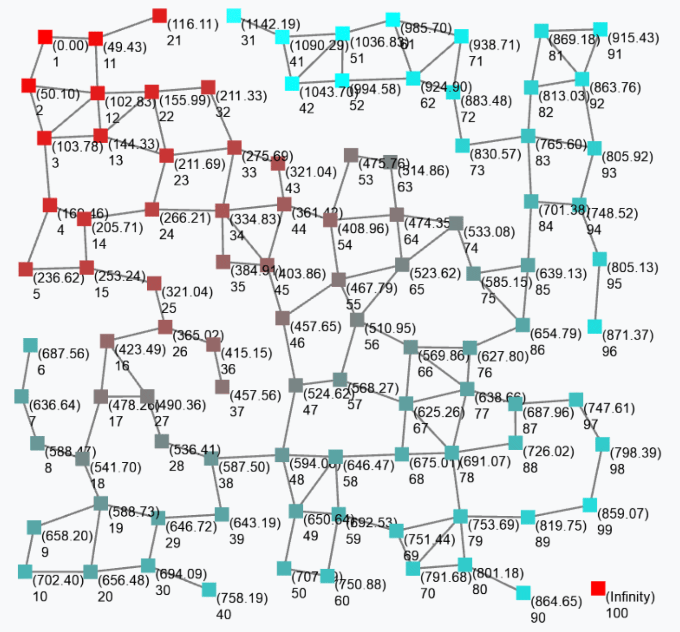
\includegraphics[width=\linewidth]{figures/gradient-example.png}
    \caption
    {
        A graphical representation of a gradient after stabilization.
        %
        Each device of the network is labelled with its distance from the source (in parenthesis) and its ID.
        %
        The source device is the one with ID 1.
        %
        Note that devices that are not connected to the source are considered to be at an infinite distance from it.
    }
    \label{fig:gradient}
\end{figure}
%
The implementation of a gradient using ScaFi is presented below.
%
\begin{lstlisting}[frame=single, language=scala]
def gradient(src: Boolean): Double =
  rep(Double.PositiveInfinity) { distance =>
    mux(src) {
      0.0
    } {
      minHoodPlus(nbr(distance) + nbrRange)
    }
  }
\end{lstlisting}
%
Some notes about the implementation:
%
\begin{itemize}
    \item \texttt{src} is an input field of source devices;
    \item the \texttt{mux} operator acts like an if statement where both branches get evaluated (unlike the \texttt{branch} construct, that only evaluates the side selected by the condition); this means that both source and non-source nodes will be aligned regardless of the chosen branch;
    \item \texttt{minHoodPlus} is an operator implemented in terms of \texttt{foldhood}, finding the minimum value for the given expression among neighbors;
    \item the \texttt{Plus} suffix of \texttt{minHood} indicates that the device itself is not considered during the calculation of the minimum, which for the gradient has the effect of preventing devices from getting stuck on low values after a source gets deactivated;
    \item \texttt{nbrRange} is a built-in neighboring sensor (implemented in terms of \texttt{nbrvar}) returning the estimated distance to the neighbor against which it is evaluated;
    \item source devices are at distance 0 from themselves, therefore the \quotes{then} branch of \texttt{mux} returns \texttt{0.0};
    \item at each device the gradient is calculated by repeatedly minimizing, for every neighbor, the sum of its currently estimated distance from the source (\texttt{nbr(distance)}) and the distance between the device and the neighbor (\texttt{nbrRange}).
\end{itemize}

\section{Proposed model}
\label{sec:proposed-model}

As stated before, in order to overcome the limitations of the proactive model this thesis proposes an approach based on \textit{reactivity}, leveraging the power of FRP (\Cref{sec:frp}) to deal with the complexity of the approach.
%
The sections below illustrate the objectives that are expected to be fulfilled by the final implementation and a high level description of the proposed reactive model.

\subsection{Objectives}

The high level goal of this thesis is to provide a model that is expressive enough to allow developers to declaratively describe \textit{self-organizing} aggregate computations, while treating the dynamics and timing of relevant events as first class citizens.
%
This vision can be in fact summarized with \textit{functional reactive self-organization}.

The main objectives to be pursued in order to accomplish the goal are:
%
\begin{itemize}
    \item \textbf{Compute only upon relevant changes}: computations should occur reactively only when something changes in the environment, in order to avoid wasteful resources usage;
    \item \textbf{Broadcast messages only upon relevant changes}: each device should avoid broadcasting an export that didn't change since the last one;
    \item \textbf{Avoid re-evaluation of unaffected sub-computations}: if a portion of the computation depends on data that didn't change, it should not be re-evaluated.
\end{itemize}

\subsection{Reactive model}

The main difference between the model proposed by this thesis and the one proposed by field calculus is the \textit{absence of computation rounds}.
%
This is dictated by the fact that one of the objectives is to have computation run only upon relevant changes in the environment, namely:
%
\begin{itemize}
    \item a new device enters the neighborhood;
    \item a device leaves the neighborhood;
    \item an export coming from a neighbor is received;
    \item the value of a sensor changes;
    \item the value of a neighboring sensor changes.
\end{itemize}
%
Previously, these sources of events were all handled in the \textit{sense} stage of a computation round, and were all collected together in order to construct the \textit{context} for the round itself.
%
However, this wasn't done in a reactive fashion, since all these events were queued up while the device was sleeping and handled all at once at the start of the sense phase.
%
This meant that, if no event was received between two rounds, the computation would still happen.
%
The reactive model, instead, handles events as soon as they are received by the device (and only in that occasion), and only broadcasts the corresponding export if it is different than the previous, effectively fulfilling the \quotes{compute only upon relevant changes} and \quotes{broadcast messages only upon changes} objectives.

For what concerns the last objective (i.e. avoiding re-evaluating unaffected sub-computations), the optimized propagation of changes will be delegated to the correct use of the FRP engine and discussed further in \Cref{sec:design}.

\section{Design}
\label{sec:design}

This section analyzes the key elements of the prototypal design for the reactive model.
%
Note that at this stage, the discussion is not tied to any particular technology, framework o programming language.
%
There is, however, a reference to Sodium's terminology and backing model, since the model uses the concept of a \textit{cell}.

\Cref{fig:class-diagram} shows an holistic picture of the proposed design, formalized as a UML class diagram.
%
\begin{figure}
    \centering
    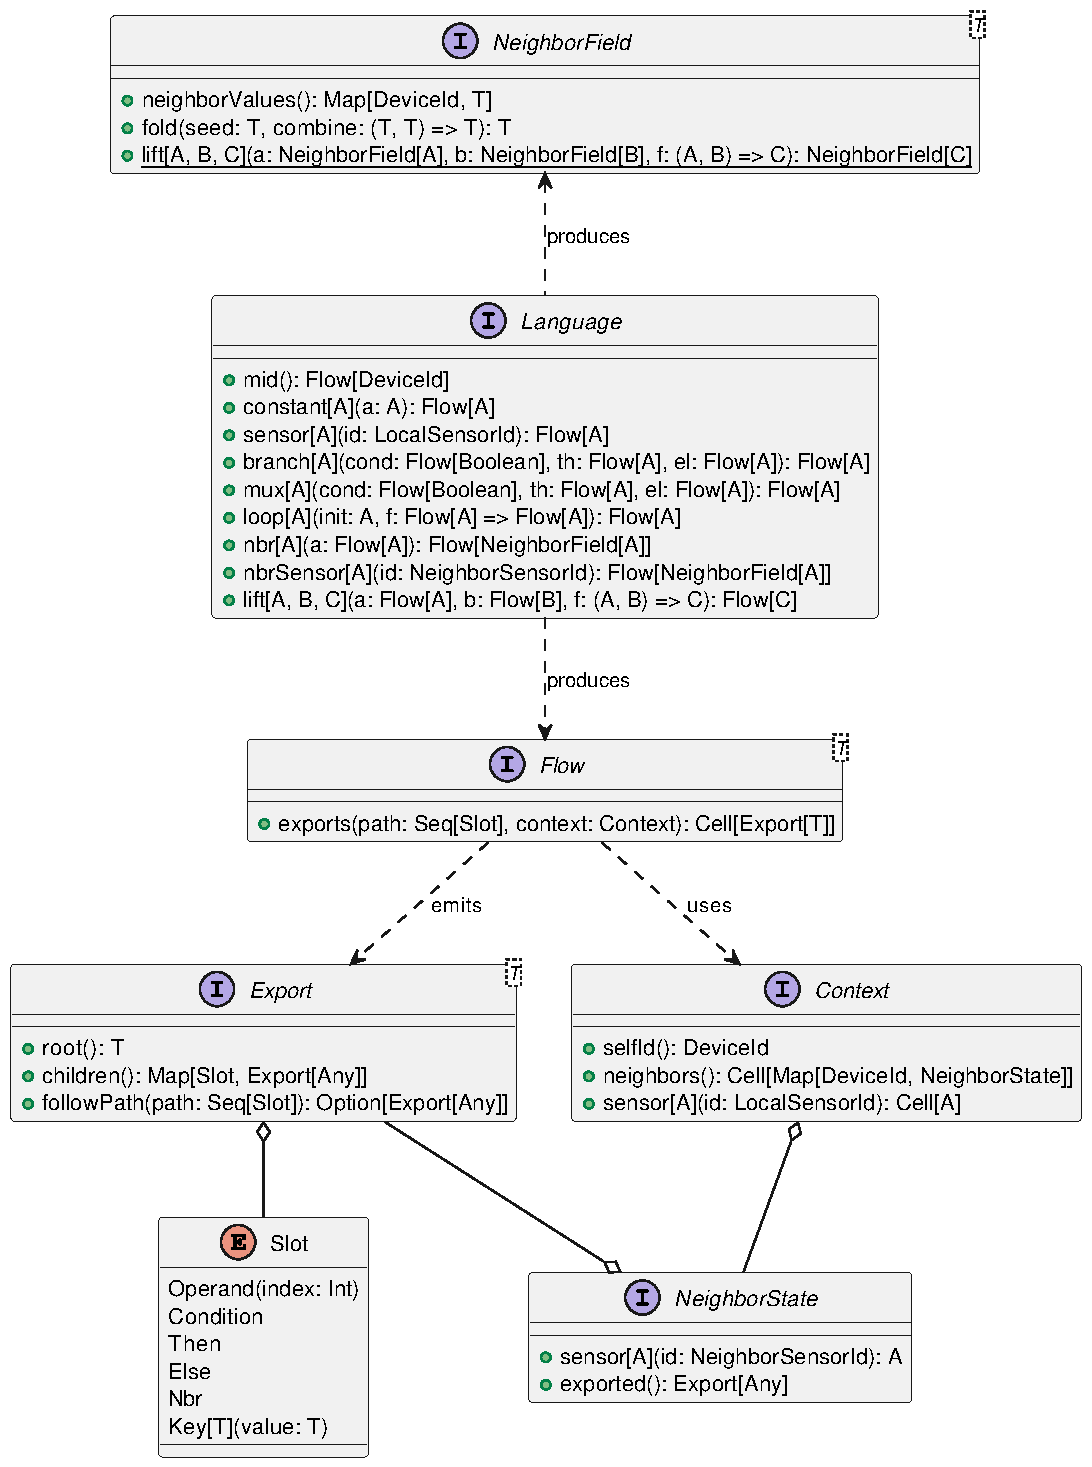
\includegraphics[width=\linewidth]{figures/diagrams/design.pdf}
    \caption{A class diagram of the reactive model.}
    \label{fig:class-diagram}
\end{figure}

% flow
% reified neighbor field
% context
% primitives
%   mid
%   loop
%   sensor
%   branch
%   nbr
%   nbrSensor
